\documentclass[aspectratio=169, 10pt]{beamer}
\usetheme{metropolis}
\usepackage{tikz}
\usetikzlibrary{calc, arrows.meta, shapes.geometric}

\title{Engineering Curves: Construction of Hypocycloid}
\subtitle{Rolling Circle on Interior of Fixed Circle with Tangent \& Normal}
\author{Gajavada Sanjeevkumar}
\date{}

\metroset{numbering=none}

\newcommand{\stepnum}{0}
\setbeamercolor{custom footer}{fg=white, bg=black!80}

\setbeamertemplate{footline}{%
  \leavevmode%
  \hbox{%
    \begin{beamercolorbox}[wd=\paperwidth, ht=3.2ex, dp=1.4ex, leftskip=1cm, rightskip=1cm]{custom footer}%
      \tiny \insertauthor \quad|\quad \inserttitle \hfill
      \ifnum\value{framenumber}=1 \textit{Introduction}%
      \else\ifnum\value{framenumber}=2 \textit{Problem Statement}%
      \else \stepnum \fi\fi
    \end{beamercolorbox}%
  }%
}
\setbeamertemplate{navigation symbols}{}

\tikzset{
  axis line/.style={thin, dash pattern=on 6pt off 2pt on 1.5pt off 2pt, black!75}, 
  directrix line/.style={ultra thick, magenta!90!black},
  construction line/.style={thin, blue!60!black},
  arc line/.style={thin, dashed, red!85!black},
  main curve/.style={ultra thick, magenta!90!black},
  tangent line/.style={thick, green!50!black},
  normal line/.style={thick, orange!80!black},
  >=Stealth,
}

\newcommand{\drawLegendCard}[1]{
  \node[draw=gray!50, fill=white, rounded corners=4pt, inner sep=4pt, anchor=north east] at (21.85, 8.5) {
    \scriptsize
    \begin{tabular}{l@{\,$\rightarrow$\,}l} #1 \end{tabular}
  };
}

\begin{document}

\begin{frame}
  \titlepage
\end{frame}

\begin{frame}{Problem Statement}
  \vfill
  \begin{block}{Question}
    \vspace{0.8em}
    Draw a \textbf{hypocycloid} generated by a rolling circle of diameter $d = 30\text{ mm}$ rolling on the inside of a fixed base circle of diameter $D = 90\text{ mm}$ for one complete revolution.
    \vspace{0.8em}
    Construct a \textbf{tangent} and a \textbf{normal} at any point $P$ on the curve.
  \end{block}
  \vfill
\end{frame}

\renewcommand{\stepnum}{1}
\begin{frame}{Step 1: Draw Fixed Base Circle \& Internal Rolling Circle}
\centering
\begin{tikzpicture}[scale=0.45]
  \useasboundingbox (-8.5,-8.5) rectangle (18.85,10.0);
  \drawLegendCard{ \textbf{Base Circle} & Radius $R = 45$ \\ \textbf{Rolling Circle} & Radius $r = 15$ }
  \coordinate (O) at (0,0);
  \draw[thick, blue!80!black] (O) circle (4.5);
  \fill[red!80!black] (O) circle (3.5pt) node[below left] {$O$};
  \coordinate (C0) at (0,3.0);
  \draw[thick, blue!80!black] (C0) circle (1.5);
  \fill[red!80!black] (C0) circle (3.5pt) node[above] {$C_0$};
  \draw[axis line] (0,0) -- (0,5.5);
\end{tikzpicture}
\end{frame}

\renewcommand{\stepnum}{2}
\begin{frame}{Step 2: Complete Hypocycloid Curve with Tangent \& Normal}
\centering
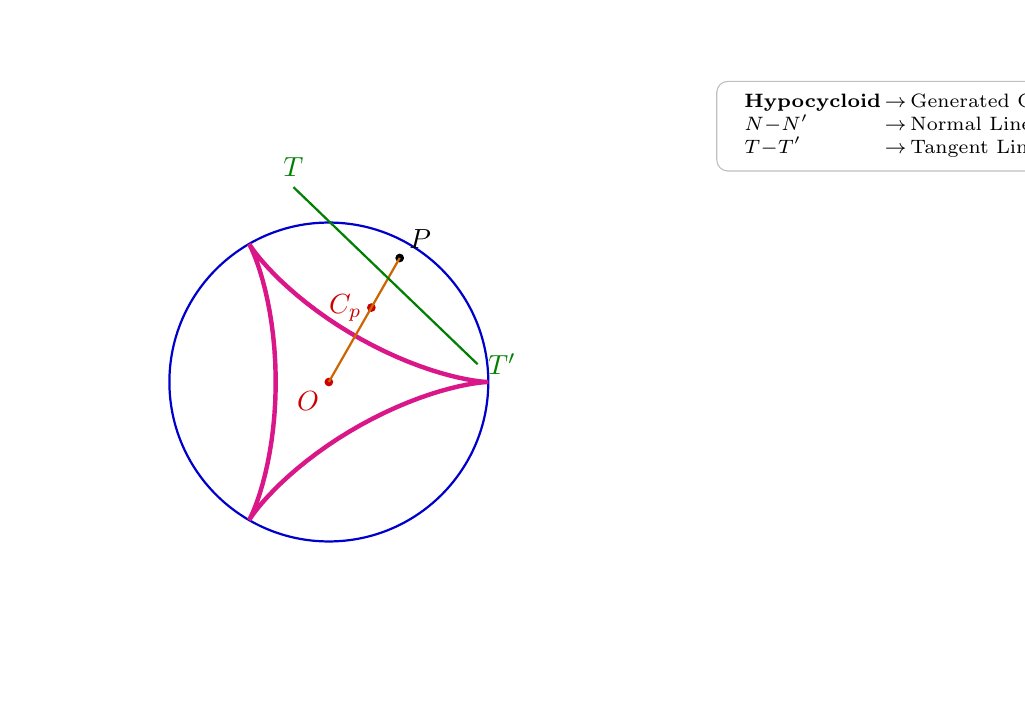
\begin{tikzpicture}[scale=0.45]
  \useasboundingbox (-8.5,-8.5) rectangle (18.85,10.0);
  \drawLegendCard{ \textbf{Hypocycloid} & Generated Curve \\ \textbf{$N\text{-}N'$} & Normal Line \\ \textbf{$T\text{-}T'$} & Tangent Line }
  \coordinate (O) at (0,0);
  \draw[thick, blue!80!black] (O) circle (4.5);
  \fill[red!80!black] (O) circle (3.5pt) node[below left] {$O$};
  
  \draw[main curve, samples=100, domain=0:6.28318] plot (
    {(4.5-1.5)*cos(\x r) + 1.5*cos((4.5-1.5)*\x / 1.5 r)},
    {(4.5-1.5)*sin(\x r) - 1.5*sin((4.5-1.5)*\x / 1.5 r)}
  );
  
  \coordinate (P) at (2.0, 3.5);
  \fill[black] (P) circle (3.5pt) node[above right] {$P$};
  \coordinate (Cp) at (1.2, 2.1);
  \draw[construction line] (P) -- (Cp);
  \fill[red!80!black] (Cp) circle (3.5pt) node[left] {$C_p$};
  \draw[normal line] (O) -- (Cp) -- (P);
  \draw[tangent line] (-1.0, 5.5) node[above] {$T$} -- (4.2, 0.5) node[right] {$T'$};
\end{tikzpicture}
\end{frame}

\end{document}
